% This file was converted to LaTeX by Writer2LaTeX ver. 1.0.2
% see http://writer2latex.sourceforge.net for more info
%\documentclass[a4paper]{article}
%\usepackage[ascii]{inputenc}
%\usepackage[T1]{fontenc}
%\usepackage[english,english]{babel}
%\usepackage{amsmath}
%\usepackage{amssymb,amsfonts,textcomp}
%\usepackage{color}
%\usepackage{array}
%\usepackage{hhline}
%\usepackage{hyperref}
%\hypersetup{pdftex, colorlinks=true, linkcolor=blue, citecolor=blue, filecolor=blue, urlcolor=blue, pdftitle=, pdfauthor=, pdfsubject=, pdfkeywords=}
%\usepackage[pdftex]{graphicx}
% Page layout (geometry)
%\setlength\voffset{-1in}
%\setlength\hoffset{-1in}
%\setlength\topmargin{2cm}
%\setlength\oddsidemargin{2cm}
%\setlength\textheight{25.7cm}
%\setlength\textwidth{17.001cm}
%\setlength\footskip{0.0cm}
%\setlength\headheight{0cm}
%\setlength\headsep{0cm}
% Footnote rule
%\setlength{\skip\footins}{0.119cm}
%\renewcommand\footnoterule{\vspace*{-0.018cm}\setlength\leftskip{0pt}\setlength\rightskip{0pt plus 1fil}\noindent\textcolor{black}{\rule{0.25\columnwidth}{0.018cm}}\vspace*{0.101cm}}
% Pages styles
%\makeatletter
%\newcommand\ps@Standard{
%  \renewcommand\@oddhead{}
%  \renewcommand\@evenhead{}
%  \renewcommand\@oddfoot{}
%  \renewcommand\@evenfoot{}
%  \renewcommand\thepage{\arabic{page}}
%}
%\makeatother
%\pagestyle{Standard}
%\title{}
%\author{}
%\date{2014-02-25T10:00:52.521000000}
%\begin{document}
\begin{uebsp}
{\centering\selectlanguage{english}\bfseries
Altes Beispiel 5.1
\par}


%\bigskip

{\selectlanguage{english}
Eine Markovkette hat die \"Ubergangswahrscheinlichkeiten}


%\bigskip

\begin{equation*}
p_{i,i+2}=p\text{ ; }p_{i,i-1}=q=1-p\text{  ;  }i\in \mathbb{Z}
\end{equation*}

%\bigskip

{\selectlanguage{english}
\index{Rekurrenz!Beispiel}
Wann ist diese Kette rekurrent? (\"Uberlegen Sie, dass die Differenzen
X(t+1) {}- X(t) unabh\"angig sind. Damit X(t) = X(0) ist, m\"ussen
doppelt so viele Schritte nach unten gemacht worden sein wie nach oben.
Damit kann man pii(t) bestimmen).}\\


\begin{center}\textbf{Lösung zu Übung 5.1}\end{center}

%\bigskip



\begin{center}
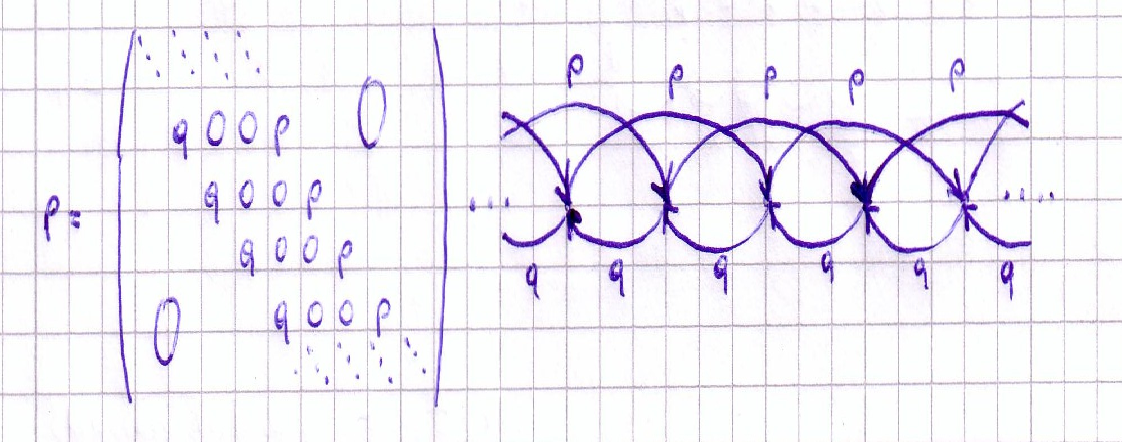
\includegraphics[width=14.825cm,height=3.706cm]{chapters/markovketten/a51Rekkurenz-img1.pdf}
\end{center}

%\bigskip


%\bigskip


%\bigskip


%\bigskip


%\bigskip


%\bigskip


%\bigskip


%\bigskip

{\selectlanguage{english}
Eine Bedingung f\"ur die Rekurrenz, die man praktisch ganz gut verwenden
kann, lautet:}


%\bigskip

\begin{equation*}
\sum _{t}p_{\mathit{ii}}(t)=\infty \text{    }(t\ge 1)
\end{equation*}

%\bigskip

{\selectlanguage{english}
 $p_{\mathit{ii}}(t)$ ist dabei nichts anderes als die
Wahrscheinlichkeit, \ in t Schritten (/Zeiten) von i nach i zu
gelangen. Da die Rekkurenz ja eine Klasseneigenschaft ist, w\"are es
egal welchen Zustand wir hier betrachten -- so k\"onnten wir 
$p_{00}(t)$ oder $p_{33}(t)$ oder sonst einen Zustand betrachten. Wir
betrachten hier (da wir die Zust\"anden nicht explizit benannt haben)
einen beliebigen Zustand i. Die \"Ubergangswahrscheinlichkeiten sind
hier eh bei jedem Zustand gleich.}


%\bigskip

{\selectlanguage{english}
Sehen wir uns einfach mal die ersten paar Glieder der Folge 
$p_{\mathit{ii}}(t)$  an. (Die Reihe bestimmen wir sp\"ater). Wir
versuchen Einfach Wege in unserem Graphen zu finden die uns von i nach
i f\"uhren und z\"ahlen dabei die Schritte.}


%\bigskip

\begin{equation*}
p_{\mathit{ii}}(1)=0
\end{equation*}
Da wir nicht in einem Schritt von unserem
Zustand wieder in unseren Zustand gelangen k\"onnen.
\begin{equation*}
p_{\mathit{ii}}(2)=0\text{ auch hier finden wir keinen Weg}
\end{equation*}
\begin{equation*}
p_{\mathit{ii}}(3)=?
\end{equation*}

%\bigskip

{\selectlanguage{english}
In 3 Schritten k\"onnen wir von i nach i gelangen. Aber daf\"ur gibt es
mehr als eine M\"oglichkeit. Denn wir k\"onnen die Permutationen von 
$\{\uparrow ,\downarrow ,\downarrow \}$ bilden. Genauer handelt es sich
hier um die Permutation einer Multimenge und wir berechnen:}


%\bigskip

\begin{equation*}
\frac{3!}{1!2!}=3=\left(\begin{matrix}3\\2\end{matrix}\right)
\end{equation*}
\begin{equation*}
p_{\mathit{ii}}(3)=\left(\begin{matrix}3\\2\end{matrix}\right)\cdot
p^{1}\cdot (1-p)^{2}
\end{equation*}

%\bigskip

\begin{equation*}
p_{\mathit{ii}}(4)=0\text{  wieder kein Weg zu finden!}
\end{equation*}

%\bigskip

\begin{equation*}
p_{\mathit{ii}}(5)=0\text{  wieder kein Weg zu finden!}
\end{equation*}

%\bigskip

\begin{equation*}
p_{\mathit{ii}}(6)=?
\end{equation*}

%\bigskip

{\selectlanguage{english}
Diesmal  $\{\uparrow ,\uparrow ,\downarrow ,\downarrow ,\downarrow
,\downarrow \}$ mit 
$\frac{6!}{2!4!}=15=\left(\begin{matrix}6\\2\end{matrix}\right)$ }


%\bigskip

\begin{equation*}
p_{\mathit{ii}}(6)=\left(\begin{matrix}6\\2\end{matrix}\right)p^{2}\cdot
(1-p)^{4}
\end{equation*}

%\bigskip

{\selectlanguage{english}
Wir k\"onnen die Vermutung aufstellen, dass es so weiter geht. }


%\bigskip

{\selectlanguage{english}
Demnach w\"are:}


%\bigskip

\begin{equation*}
p_{\mathit{ii}}(t)=\left\{\begin{matrix}\text{ 
}3|t\text{:}\left(\begin{matrix}t\\\frac{t}{3}\end{matrix}\right)\cdot
p^{\frac{t}{3}}\cdot (1-p)^{\frac{2t}{3}}\\3\nmid t\text{:  
}0\end{matrix}\right.
\end{equation*}
{\selectlanguage{english}
Wir wollen nun also zeigen, dass:}


%\bigskip

\begin{equation*}
\sum _{t}p_{\mathit{ii}}(t)=\infty \text{    }(t\ge 1)
\end{equation*}

%\bigskip

{\selectlanguage{english}
Wir setzen  $t=3k$ und berechnen:}


%\bigskip

\begin{equation*}
\sum _{k>0}\left(\begin{matrix}3k\\k\end{matrix}\right)\cdot p^{k}\cdot
(1-p)^{2k}=\frac{(3k)!}{k!\cdot (2k)!}\cdot p^{k}\cdot (1-p)^{2k}
\end{equation*}
{\selectlanguage{english}
Was hier hilfreich ist (auch wenn es im ersten Moment vl. \ nicht so
aussieht) ist die Stirling-Formel:}


%\bigskip

\begin{equation*}
n!\simeq \sqrt{2\pi n}\cdot (\frac{n}{e})^{n},\text{   f\"ur
}n\rightarrow \infty 
\end{equation*}

%\bigskip

{\selectlanguage{english}
Ersetzen wir unsere Fakult\"aten durch die Alternativen der
Stirling-Formel, dann k\"urzt sich letztendlich viel Weg ung es bleibt
schlie{\ss}lich:}


%\bigskip

\begin{equation*}
\sum _{k>0}\sqrt{\frac{3}{4\pi k}}\cdot
\left(\frac{27}{4}\right)^{k}\cdot p^{k}\cdot
(1-p)^{2k}=\sqrt{\frac{3}{4\pi }}\cdot \sum
_{k>0}\sqrt{\frac{1}{k}}\cdot \left(\frac{27}{4}\right)^{k}\cdot
p^{k}\cdot (1-p)^{2k}
\end{equation*}
{\selectlanguage{english}
Was hilft uns das?}


%\bigskip

{\selectlanguage{english}
Wir wissen, dass}

\begin{equation*}
\sum _{k>0}{\frac{1}{\sqrt{k}}}=\infty 
\end{equation*}
{\selectlanguage{english}
Damit gilt auch  $\sum _{k>0}{\frac{1}{\sqrt{k}}}\cdot 1=\infty $ also
wenn:}

\begin{equation*}
\left(\frac{27}{4}\right)^{k}\cdot p^{k}\cdot (1-p)^{2k}\ge 1\rightarrow
(\left(\frac{27}{4}\right)\cdot p\cdot (1-p)^{2})^{k}\ge 1\rightarrow
\left(\frac{27}{4}\right)\cdot p\cdot (1-p)^{2}\ge 1
\end{equation*}

%\bigskip

{\selectlanguage{english}
ist die Kette sicher rekurrent!}


%\bigskip

{\selectlanguage{english}
Aus der L\"osung der resultierenden Ungleichung 
$p^{3}-2p^{2}+p-\frac{4}{27}\ge 0$ ergeben sich die L\"osungen:}


%\bigskip

{\selectlanguage{english}
 $p=\frac{1}{3}$ und  $p\ge \frac{4}{3}$  womit wir die eindeutige
L\"osung  $p=\frac{1}{3}$ gefunden haben, denn die Wahrscheinlichkeit
kann nie gr\"o{\ss}er 1 sein!}



%\end{document}
\end{uebsp}
